\newpage
\chapter{Diskussion}
Bla bla. \\

Dette projekt valgte vi at dele op i en række delmål. Delmålene var delt op i grupperne Basics, Advanced, Brikker, Helhedsindtryk og Hardware. Basics var det der skulle til for at få et fungerende spil og de efterfølgende mål har skullet opfylde vores ønsker om at lave et realistisk spil med godt gameplay. Ud fra disse delmål, samt det ekstra mål at man skulle kunne få powerups i spillet, lavede vi tidsplanen vist på Figur \ref{fig:tidsplan2}, øverst. Som det kan ses nederst på samme figur, tog implementeringen af brikkerne dog væsentlig længere tid end forventet og det gjorde at vi ikke nåede vores mål om at lave powerups. Årsagen til dette var, at vi sammen med de avancerede delmål valgte at gøre bolden større. Da vi skiftede til terminalen putty i stedet for HyperTerminal og fik mulighed for at køre terminalen i fuldskærm valgte vi at lave bolden $4\times2$ karakterer. Dette gjorde at bolden kunne ramme flere brikker af gangen og briklogikken blev af den grund meget mere kompleks, se flowchartet på Figur \ref{fig:brickFlow} og  Appendix \nameref{reflexball} linje 145 og frem. En yderligere udfordring var at bolden bevægede sig to karakterer af gangen i x-retningen på skærmen. Der kunne derfor komme en stor del af bolden ind i brikkerne, hvilket også vanskeliggjorde at fastslå hvordan brikken var blevet ramt af bolden. \\ 
En stor del af arbejdet med brikkerne bestod derfor af debugging og rettelser i koden. For at teste briklogikken skrev vi tekst ud på skærmen der fortalte os hvordan vi havde ramt brikkerne, om flagene \texttt{dontDeflectX} og \dontDeflectY} var blevet sat og om det var detekteret at der var brikker ved siden af og over/under den ramte brik. På den måde kunne vi finde præcis de steder i koden hvor der var problemer med vores logik. 


Skriv verifikationsafsnit
	Globale variabler
	Problemer med brikker og bold
	Nåede ikke power-ups og power-downs
	Fandt undervejs ud af vi ville inkludere ASCII-Art
	Hvad vi nåede og hvad vi ikke nåede (se tidsplan2.png
	Hvordan vi har testet det hele


\begin{figure}[h!]
\centering
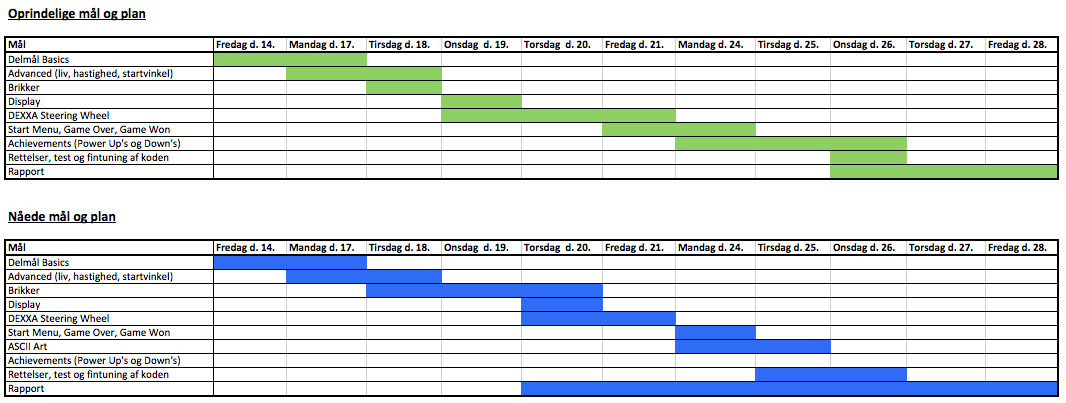
\includegraphics[scale=0.4]{figs/Tidsplan2.png}
\caption{Øverst: Tidsplan over de forskellige delmål og hvornår de skulle være færdige. Nederst: Hvad vi rent faktisk lavede og hvornår}
\label{fig:tidsplan2}
\end{figure}